\documentclass[11pt]{article}
\usepackage{latexsym}
\usepackage{amsmath}
\usepackage{amssymb}
\usepackage{amsthm}
\usepackage{epsfig}
\usepackage{dsfont}
\usepackage[tight]{subfigure}
\setcounter{secnumdepth}{4}
\bibliographystyle{ieeetr}


\usepackage{amsmath}

\DeclareMathOperator*{\minimize}{min}
\DeclareMathOperator*{\maximize}{max}

\usepackage{algorithm}
 %on linux you may need to run sudo apt-get install texlive-full to install algorithm.sys
\usepackage{algorithmic}

\usepackage{verbatim}

\newcommand{\handout}[5]{
  \noindent
  \begin{center}
  \framebox{
    \vbox{
      \hbox to 5.78in { {#1} \hfill #2 }
      \vspace{4mm}
      \hbox to 5.78in { {\Large \hfill #5  \hfill} }
      \vspace{2mm}
      \hbox to 5.78in { {\em #3 \hfill #4} }
    }
  }
  \end{center}
  \vspace*{4mm}
}

\newcommand{\lecture}[5]{\handout{#1}{#2}{#3}{#4}{#5}}
\newcommand{\collision}[0]{\mathrm{collision}}
\newcommand{\nocollision}[0]{\overline{\collision}}

\newcommand*{\QED}{\hfill\ensuremath{\square}}

\newtheorem{theorem}{Theorem}
\newtheorem{corollary}[theorem]{Corollary}
\newtheorem{lemma}[theorem]{Lemma}
\newtheorem{observation}[theorem]{Observation}
\newtheorem{proposition}[theorem]{Proposition}
\newtheorem{definition}[theorem]{Definition}
\newtheorem{claim}[theorem]{Claim}
\newtheorem{fact}[theorem]{Fact}
\newtheorem{assumption}[theorem]{Assumption}
\newtheorem{note}[theorem]{Note}

% 1-inch margins, from fullpage.sty by H.Partl, Version 2, Dec. 15, 1988.
\topmargin 0pt
\advance \topmargin by -\headheight
\advance \topmargin by -\headsep
\textheight 8.9in
\oddsidemargin 0pt
\evensidemargin \oddsidemargin
\marginparwidth 0.5in
\textwidth 6.5in

\parindent 0in
\parskip 1.5ex
%\renewcommand{\baselinestretch}{1.25}

\begin{document}

\lecture{Statistical Techniques in Robotics (16-831, S22)}{Lecture \#15
  (Wednesday, March 16)}{Lecturer: Alex LaGrassa}{Scribes: Alex Pletta, Benjamin Younes}{Value-Based Model-Based Control}

\section{Review}
In the last lectures, we previously learned about Markov Decision Processes (MDP).

\subsection{Markov Decision Process}

A Markov Decision Process \cite{Bel} is a framework for modeling how an agent can decide to take actions in given states to obtain a reward.

\subsubsection{Notation Definition}

\begin{align*}
    &s \in \mathcal{S} & \text{State} \\
    &a \in \matchal{A}_s & \text{Action} \\ 
    &p(s'|s,a) & \text{State transition dynamic} \\
    &r(s', s, s) & \text{Reward function (general case)} \\
    &p_0(s) & \text{State prior} \\
    &\pi(a|s) & \text{Policy} \\
    &\gamma & \text{Discount factor}
\end{align*}

An MDP trajectory is composed of a sequence of states and actions taken by the agent for a time horizon of $T$.

\begin{equation}
    \zeta = (s_0, a_0, s_1, a_1, ... , s_T, a_T)    
\end{equation}

One can form the probability of a state-action trajectory $p(s_0, a_0, s_1, a_1, ... , s_T, a_T)$ and an associated reward probability of that trajectory $r(s_0, a_0, s_1, a_1, ... , s_T, a_T)$. This can be factorized in many ways, most traditionally as the following:

The traditional probability factorization is:
\begin{equation}
    p(s_0, a_0, s_1, a_1, ... , s_T, a_T) = p_0(s_0) \prod_t p(s_{t+1}|s_t, a_t) p(a_t|s_t)
\end{equation}

where $p_0(s_0)$ is the prior state, $p(s_{t+1}|s_t, a_t)$ is the state transition dynamic, and $p(a_t|s_t)$ is the policy.

The traditional reward factorization can take several forms, including:
\begin{enumerate}
\item Reward as a function of the previous state, current state, and action
\begin{equation}
    r(s_0, a_0, s_1, a_1, ... , s_T, a_T) = r(s_0, a_0, s_1) + r(s_1, a_1, s_2) + ...
\end{equation}

\item Reward as a function of the previous state and action
\begin{equation}
    r(s_0, a_0, s_1, a_1, ... , s_T, a_T) = r(s_0, a_0) + r(s_1, a_1) + ... 
\end{equation}

\item Reward as a function of the state
\begin{equation}
    r(s_0, a_0, s_1, a_1, ... , s_T, a_T) = r(s_0) + r(s_1) + ... 
\end{equation}
\end{enumerate}

An MDP policy $\pi(a|s)$ is a strategy of selecting actions at each state that result in a trajectory. The state transition dynamic describes the likelihood of arriving at a certain state after following a certain action. This captures the unmodeled system dynamics, such as those introduced by disturbances, that could lead to a transition to an unexpected state. The state transition dynamic $p(s'|s,a)$ is the probability of arriving at state $s'$ after taking action $a$ at state $s$.

An MDP reward performance can be evaluated using the state value function, which is the sum of total expected reward over a trajectory from following a policy $\pi$ for starting in a state $s_0$. Note that each reward is calculated depending on the selected factorization. The factorization is based on the Markov assumptions inherent in MDP problems.

\begin{equation}
    V^{\pi}(s) = \mathbb{E}_p [r_0 + r_1 + ... | s_0 = s]
\end{equation}

The value function can be defined over different reward horizons:

\begin{enumerate}
    \item Infinite horizon return
    \begin{equation}
        V^{\pi}(s) = \mathbb{E}_p [r_0 + r_1 + ... | s_0 = s]
    \end{equation}
    \item Finite horizon return
    \begin{equation}
        V^{\pi}(s) = \mathbb{E}_p [r_0 + r_1 + ... + r_T | s_0 = s]
    \end{equation}
    \item Infinite horizon discounted return
    \begin{equation}
        V^{\pi}(s) = \mathbb{E}_p [r_0 + \gamma r_1 + \gamma^2 r_2+  ... | s_0 = s]
    \end{equation}
\end{enumerate}

The most common reward horizon is the infinite horizon discounted return, with a discount factor $\gamma$ that typically is $\gamma \in [0.9, 0.99]$.

The MDP reward performance can also be defined using the State-Action Value Function. The State-Action Value Function defines the expected return of a trajectory given an initial state $s$ and initial action $a$ with a policy $\pi$. This function assumes the action $a$ is taken at state $s$ and then the policy $\pi$ is followed for the rest of the trajectory. Within the infinite horizon discounted return formulation, the State-Action Value Function can be written as:

\begin{equation}
    Q^{\pi}(s,a) = \mathbb{E}_p [r(s_0) + \gamma r(s_1) + \gamma^2 r(s_2) +  ... | s_0 = s, a_0 = a]
\end{equation}

The relationship between the Value Function and State-Action Value Function is linked by the sum over the possible initial actions with the given policy:

\begin{equation}
    V^{\pi}(s) = \sum_a \pi(a|s) Q^{\pi}(s,a)
\end{equation}

%This section serves as a review of the previous lecture and any other context required to frame the content of the current lecture. 

%You may format the scribes in any way you like, aside from changing font style, size and page format. Please use subsections and paragraphs to increase the readability of your notes.

%Length requirement 1-2 pages.

\section{Summary}


In today's lecture, we discussed the relationship between MDP's and closed-loop control to find optimal policies for a given task through policy iteration and value iteration. In class we covered an example that used a tabular environment with discrete states and actions (e.g. a checkerboard where the agent can move up, down, left, right, or stay in-place), but the concept of MDP's and optimal policies extend to continuous representations as well. 


\subsection{Open Loop vs. Closed Loop Control Brief Summary}
In class we used open vs. closed loop control with a visual demonstration of pouring a proper amount of liquid into a glass. The demonstration was structured such that the lecturer was given two attempts to pour liquid into the glass, where the open loop case did not have visual feedback (the lecturer had their eyes closed) and the closed loop case did have visual feedback (the lecturer had their eyes open).

This demonstrated that open loop control can have reasonably good performance it the model of the environment is good, but that closed loop control is more robust and can often be much more accurate. In the context of reinforcement learning, we will use closed loop control to update our model after receiving reward feedback from the environment.

\subsection{Bellman Equation}
The Bellman Equation is a recursive dynamic programming equation that derives the optimal reward over all actions that could be taken at a given state \cite{doi:10.1073/pnas.38.8.716}. This equation is defined as the following for a given policy $\pi$.

\begin{equation}
    V^{\pi}(s) = \sum_{a\in \mathcal{A}} \pi(a|s) \sum_{s'\in \mathcal{S}} P(s'|s,a)(R(s,a)+\gamma V^{\pi}(s'))
\end{equation}

The Bellman Optimality Equation is a special form of the Bellman Equation that holds for the \textit{optimal} policy $\pi^*$ that maximizes the expected reward.

\begin{equation}
    V^{\pi^*}(s) = \text{max}_a \sum_{s'} P(s'|s,a)(R(s,a)+\gamma V^{\pi^*}(s'))
\end{equation}

We will use the Bellman Optimality Equation to solve for optimal policies given states through both policy and value iteration. 

\subsection{Model-Based Value-Based Control}

We will model and update our system using closed loop control over both policy and value iteration. In both approaches, we will continuously loop over all states and improve our policy. Our control loop will cycle back and forth between a prediction stage and then an evaluation stage. 

\begin{figure}[!ht]
\centering
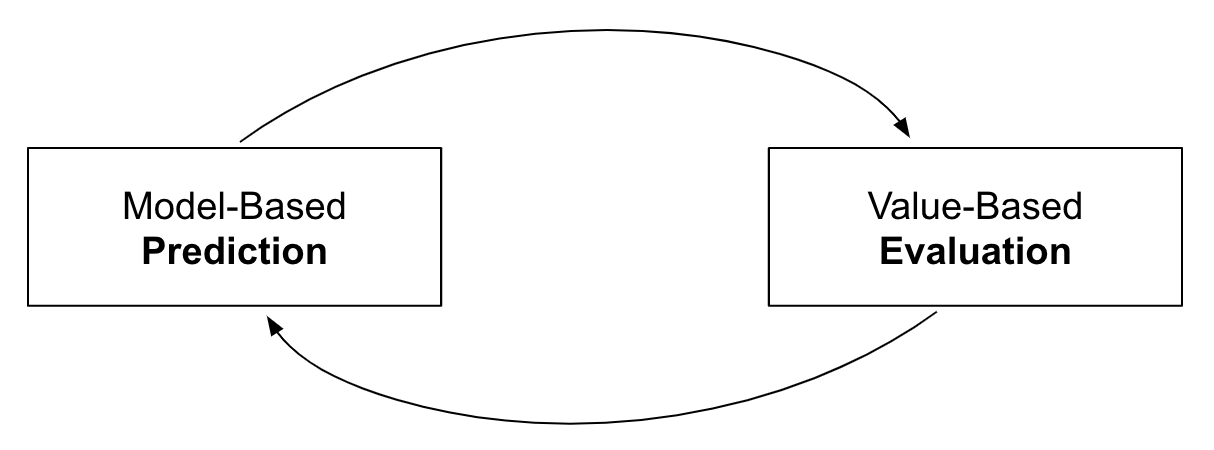
\includegraphics[width=0.7\linewidth]{Lecture_15/control_loop.png}
\caption{Model-Based Value-Based Closed-Loop Control.}
\end{figure}

\subsubsection{Policy Iteration}
In Policy Iteration \cite{Bel}, the agent evaluates the value $V$ or action value $Q$ for a given policy, and then improves the policy using the value $V$ or action value $Q$. 

\begin{figure}[!ht]
\centering
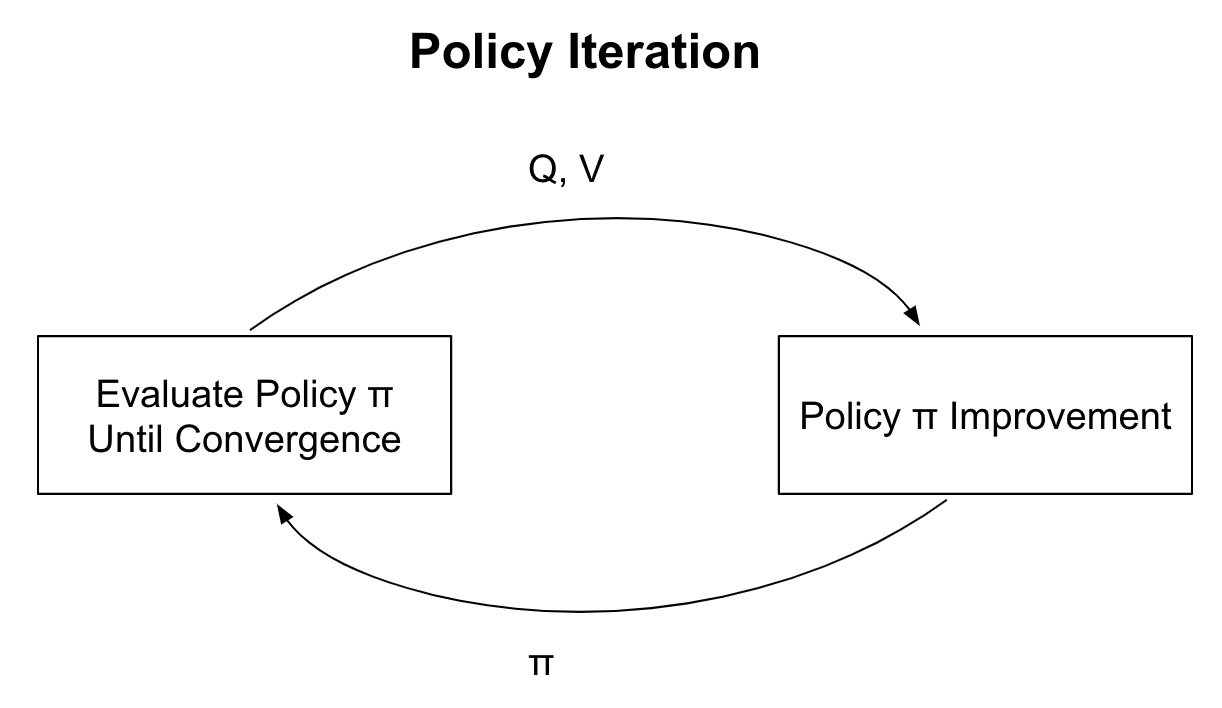
\includegraphics[width=0.7\linewidth]{Lecture_15/policy_iteration.png}
\caption{Policy Iteration Closed-Loop Control.}
\end{figure}

\begin{itemize}
    \item \underline{Evaluation:}
    The iterations begin with a random policy $\pi$. This policy is then evaluated over all states. Note that the policy evaluation needs to be repeated until the values are stable for that policy. 
    \item \underline{Improvement:}
    The policy actions are then updated using the calculated values.
\end{itemize}

This control loop iterates between evaluation and policy improvement updates until convergence, which occurs when the policy stays the same within some threshold $\eplison$ according to Algorithm \ref{algo:policy} below.

\begin{algorithm}[H]
\caption{Policy Iteration Algorithm}
\label{algo:policy}
\begin{algorithmic}[1]

\WHILE{$\pi$ is unchanged \hfill $\triangleright$ Loop until final policy convergence}

\STATE $V \leftarrow \text{rand}(\mathbb{R})$
\STATE $V' \leftarrow \text{rand}(\mathbb{R})$

\WHILE{$\text{max}_s |V(s) - V'(s)| \leq \epsilon$ \hfill $\triangleright$ Iterate with policy until values converge} 
\STATE $V' \leftarrow V$
\FOR{$s\in\mathcal{S}$}
    \STATE{$Q(s,a) = r(s) + \gamma \sum_{s'} p(s'|s,a)V'(s') \quad \forall a$}
    \STATE{$V(s) = \sum_{a} \pi(a|s)Q(s,a)$}
\ENDFOR
\ENDWHILE
\FOR{$s\in\mathcal{S}$ \hfill $\triangleright$ Update the policy to improve}
    \STATE $\pi(s) = \text{argmax}_a Q(s,a)$
\ENDFOR
\ENDWHILE
\end{algorithmic}
\end{algorithm}

It can be proven that the converged policy iteration algorithm will arrive at the optimal policy because every iteration improves the policy as defined in the update step. We will show this by comparing the value function $V$ to the action value function $Q$ using policy $\pi$ and updated policy $\pi'$. 

Note that as defined by the value and action value functions, $V^{\pi}(s) \leq Q^{\pi}(s,\pi')$. We can leverage this inequality to then relate $V^{\pi}(s)$ to $V^{\pi'}(s)$ by using induction over the state action pairs.

\begin{align}
    V^{\pi}(s) &\leq Q^{\pi}(s,\pi') \\
    &= \mathbb{E}_a [r(s,a) + \gamma V^{\pi}(s')] \\
    &\leq \mathbb{E}_a [r(s,a) + \gamma Q^{\pi}(s',\pi')] \\
    &= \mathbb{E}_{a,a'} [r(s,a) + \gamma r(s',a') + \gamma^2 V^{\pi}(s'')] \\
    &\leq ... \\
    &\leq \mathbb{E}_{a,a',a''} [r(s,a) + \gamma r(s',a') + \gamma^2 r(s'', a'') + ...] \\
    &= V^{\pi'}(s)
\end{align}

We can then say that

\begin{equation}
    V^{\pi}(s) &\leq V^{\pi'}(s)
\end{equation}

so each iteration of the policy update will produce a new policy that has a value that is at least as good as the previous policy. Therefore, once the policy converges to a stable policy that final policy will be the optimal policy.

\hfill $\blacksquare$


\subsubsection{Value Iteration}
In Value Iteration \cite{Bel}, the value $V$ or action value $Q$ and the policy $\pi$ are calculated at the same time. The policy $\pi$ and the state values are initialized randomly. 

\begin{figure}[!ht]
\centering
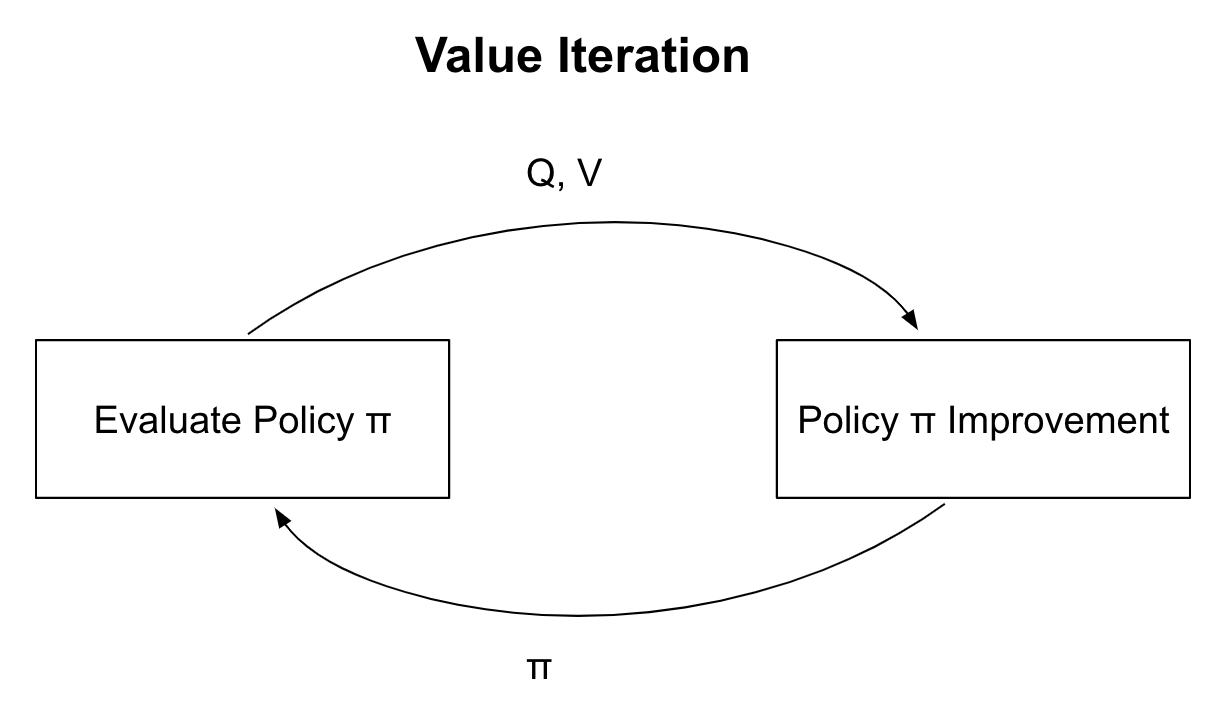
\includegraphics[width=0.7\linewidth]{Lecture_15/value_iteration.png}
\caption{Value Iteration Closed-Loop Control.}
\end{figure}

\begin{itemize}
    \item \underline{Evaluation:}
    The evaluation step calculates the value function using the current best action for each state.
    \item \underline{Improvement:}
    The improvement step takes the best action from each state that maximizes the Bellman Optimality Equation.
\end{itemize}

The value iteration algorithm (Algorithm \ref{algo:value}) repeats until the values for each state no longer change. At this point the actions in each state are the optimal policy, because each action was calculated using the Bellman Optimality Equation.




\begin{algorithm}[H]
\caption{Value Iteration Algorithm}
\label{algo:value}
\begin{algorithmic}[1]


\STATE $\pi \leftarrow \mathbf{\mathcal{A}}$
\STATE $V \leftarrow \text{rand}(\mathbb{R})$
\STATE $V' \leftarrow \text{rand}(\mathbb{R})$

\WHILE{$\text{max}_s |V(s) - V'(s)| \leq \epsilon$ \hfill $\triangleright$ Iterate until values converge} 
\STATE $V' \leftarrow V$
\FOR{$s\in\mathcal{S}$}
    \STATE{$Q(s,a) = r(s) + \gamma \sum_{s'} p(s'|s,a)V'(s') \quad \forall a$}
    \STATE $\pi(s)=\text{argmax}_a Q(s,a)$
    \STATE{$V(s) = Q(s,\pi(s))$} \hfill $\triangleright$ Update values
\ENDFOR
\ENDWHILE

\end{algorithmic}
\end{algorithm}

\subsection{Policy vs. Value Iteration Takeaways}

As seen, policy and value iteration both converge to the optimal policy. The selection to use one approach vs. the other depends on the problem being solved. General guidelines are that value iteration can typically converge faster, unless it is very expensive to compute the value $V$ and action value $Q$. In this case, it may be faster to use policy iteration. 

In the real-world, additional challenges can be that the problem may only be partially observable and that the system dynamics may not be modeled perfectly. However, the optimal policy can still often be discovered even with modeling imperfections, thanks to the closed-loop control architecture.

\subsection{Connection to Reinforcement Learning}
Although not covered directly in the lecture, we will now make the connection between the model-based value-based control and reinforcement learning (RL). We have been discussing our control loop in terms of an agent making an action and receiving a reward. We covered how to use policy and value iteration in combination with the Bellman Equation and Bellman Optimality Equation to find an optimal policy, with given transition dynamic and reward. We used a closed-loop control feedback to use this reward in the updating steps of the iterations. 

In our formulation, we used a state transition dynamic and model of which state-action pairs would result in certain amounts of reward. This can also be called Model-Based RL, but reinforcement learning can be formulated in such a way that the agent does not necessarily need to use the transition dynamics and/or reward, as long as the agent finds some policy, in so-called Model-Free RL. In Model-Based RL, the agent leverages it's knowledge of the environment and reward model to improve the reward from its policy faster and more accurately. However, in Model-Free RL the agent can compute its policy using only the reward from that policy directly with no other modeling understanding. This can be more flexible to unknown or changing dynamics but can also be more challenging to train.

\begin{figure}[!ht]
\centering
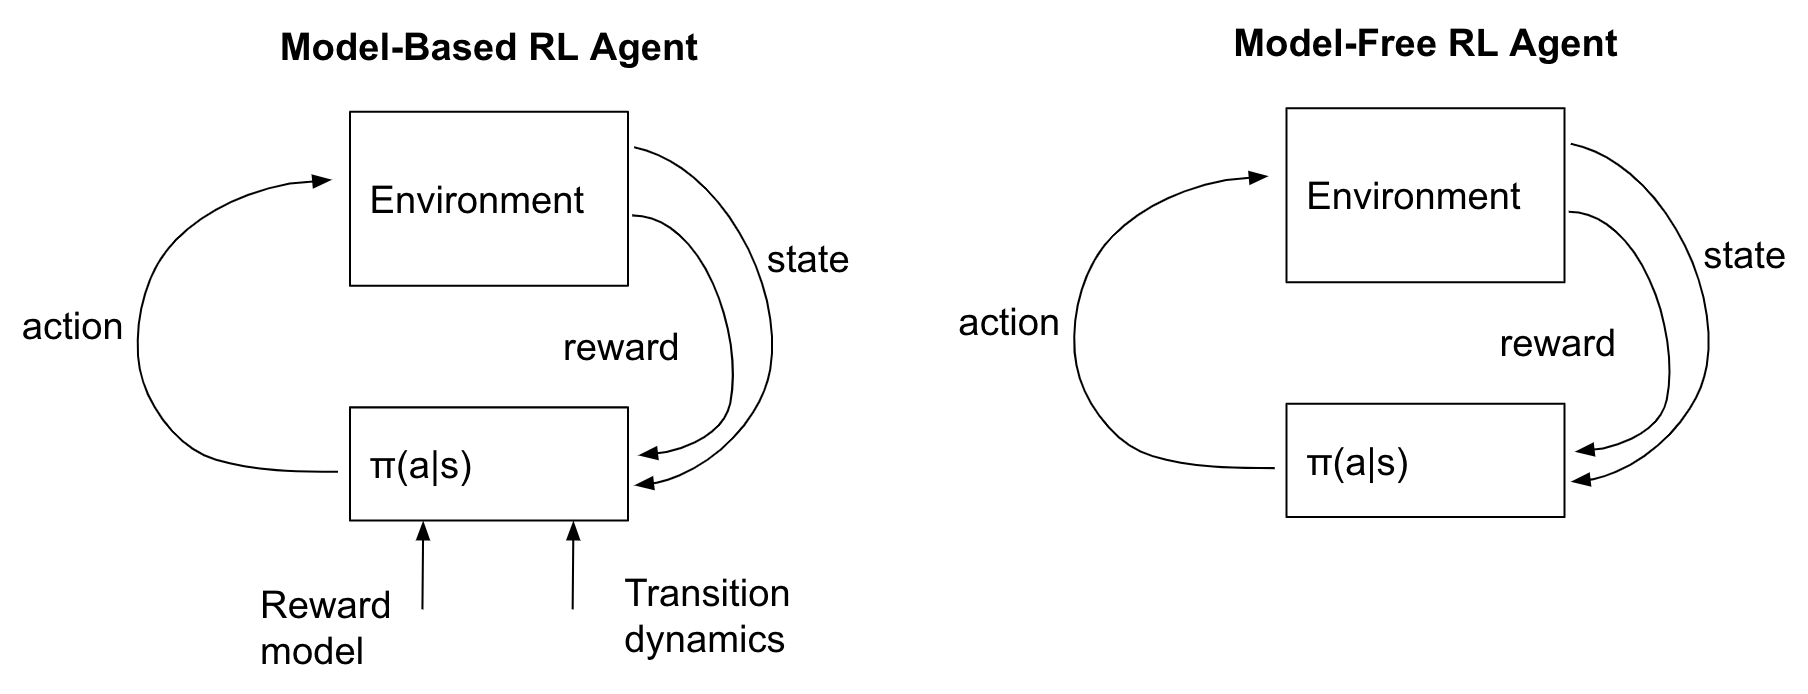
\includegraphics[width=0.7\linewidth]{Lecture_15/model_rl.png}
\caption{Model-Based vs. Model-Free Reinforcement Learning.}
\end{figure}

%\section*{References}
%Include your references here. Please cite any resources you found useful.	
%Populate the refs.bib file or list your references manually. Be consistent in formatting!
\vspace*{\fill}
{
\bibliography{refs}
\bibliographystyle{abbrv}
}

%\section{Appendix}
%This section provides any relevant background material that was not covered in the lectures, but was found to be useful for understanding the material. 
%For example, derivations, theory underlying techniques employed, etc. 

%Additionally, this section can summarizes applications or extensions of these techniques found in the literature. 

\end{document} % Done!


